% Options for packages loaded elsewhere
\PassOptionsToPackage{unicode}{hyperref}
\PassOptionsToPackage{hyphens}{url}
%
\documentclass[
]{article}
\usepackage{amsmath,amssymb}
\usepackage{iftex}
\ifPDFTeX
  \usepackage[T1]{fontenc}
  \usepackage[utf8]{inputenc}
  \usepackage{textcomp} % provide euro and other symbols
\else % if luatex or xetex
  \usepackage{unicode-math} % this also loads fontspec
  \defaultfontfeatures{Scale=MatchLowercase}
  \defaultfontfeatures[\rmfamily]{Ligatures=TeX,Scale=1}
\fi
\usepackage{lmodern}
\ifPDFTeX\else
  % xetex/luatex font selection
\fi
% Use upquote if available, for straight quotes in verbatim environments
\IfFileExists{upquote.sty}{\usepackage{upquote}}{}
\IfFileExists{microtype.sty}{% use microtype if available
  \usepackage[]{microtype}
  \UseMicrotypeSet[protrusion]{basicmath} % disable protrusion for tt fonts
}{}
\makeatletter
\@ifundefined{KOMAClassName}{% if non-KOMA class
  \IfFileExists{parskip.sty}{%
    \usepackage{parskip}
  }{% else
    \setlength{\parindent}{0pt}
    \setlength{\parskip}{6pt plus 2pt minus 1pt}}
}{% if KOMA class
  \KOMAoptions{parskip=half}}
\makeatother
\usepackage{xcolor}
\usepackage[margin=1in]{geometry}
\usepackage{color}
\usepackage{fancyvrb}
\newcommand{\VerbBar}{|}
\newcommand{\VERB}{\Verb[commandchars=\\\{\}]}
\DefineVerbatimEnvironment{Highlighting}{Verbatim}{commandchars=\\\{\}}
% Add ',fontsize=\small' for more characters per line
\usepackage{framed}
\definecolor{shadecolor}{RGB}{248,248,248}
\newenvironment{Shaded}{\begin{snugshade}}{\end{snugshade}}
\newcommand{\AlertTok}[1]{\textcolor[rgb]{0.94,0.16,0.16}{#1}}
\newcommand{\AnnotationTok}[1]{\textcolor[rgb]{0.56,0.35,0.01}{\textbf{\textit{#1}}}}
\newcommand{\AttributeTok}[1]{\textcolor[rgb]{0.13,0.29,0.53}{#1}}
\newcommand{\BaseNTok}[1]{\textcolor[rgb]{0.00,0.00,0.81}{#1}}
\newcommand{\BuiltInTok}[1]{#1}
\newcommand{\CharTok}[1]{\textcolor[rgb]{0.31,0.60,0.02}{#1}}
\newcommand{\CommentTok}[1]{\textcolor[rgb]{0.56,0.35,0.01}{\textit{#1}}}
\newcommand{\CommentVarTok}[1]{\textcolor[rgb]{0.56,0.35,0.01}{\textbf{\textit{#1}}}}
\newcommand{\ConstantTok}[1]{\textcolor[rgb]{0.56,0.35,0.01}{#1}}
\newcommand{\ControlFlowTok}[1]{\textcolor[rgb]{0.13,0.29,0.53}{\textbf{#1}}}
\newcommand{\DataTypeTok}[1]{\textcolor[rgb]{0.13,0.29,0.53}{#1}}
\newcommand{\DecValTok}[1]{\textcolor[rgb]{0.00,0.00,0.81}{#1}}
\newcommand{\DocumentationTok}[1]{\textcolor[rgb]{0.56,0.35,0.01}{\textbf{\textit{#1}}}}
\newcommand{\ErrorTok}[1]{\textcolor[rgb]{0.64,0.00,0.00}{\textbf{#1}}}
\newcommand{\ExtensionTok}[1]{#1}
\newcommand{\FloatTok}[1]{\textcolor[rgb]{0.00,0.00,0.81}{#1}}
\newcommand{\FunctionTok}[1]{\textcolor[rgb]{0.13,0.29,0.53}{\textbf{#1}}}
\newcommand{\ImportTok}[1]{#1}
\newcommand{\InformationTok}[1]{\textcolor[rgb]{0.56,0.35,0.01}{\textbf{\textit{#1}}}}
\newcommand{\KeywordTok}[1]{\textcolor[rgb]{0.13,0.29,0.53}{\textbf{#1}}}
\newcommand{\NormalTok}[1]{#1}
\newcommand{\OperatorTok}[1]{\textcolor[rgb]{0.81,0.36,0.00}{\textbf{#1}}}
\newcommand{\OtherTok}[1]{\textcolor[rgb]{0.56,0.35,0.01}{#1}}
\newcommand{\PreprocessorTok}[1]{\textcolor[rgb]{0.56,0.35,0.01}{\textit{#1}}}
\newcommand{\RegionMarkerTok}[1]{#1}
\newcommand{\SpecialCharTok}[1]{\textcolor[rgb]{0.81,0.36,0.00}{\textbf{#1}}}
\newcommand{\SpecialStringTok}[1]{\textcolor[rgb]{0.31,0.60,0.02}{#1}}
\newcommand{\StringTok}[1]{\textcolor[rgb]{0.31,0.60,0.02}{#1}}
\newcommand{\VariableTok}[1]{\textcolor[rgb]{0.00,0.00,0.00}{#1}}
\newcommand{\VerbatimStringTok}[1]{\textcolor[rgb]{0.31,0.60,0.02}{#1}}
\newcommand{\WarningTok}[1]{\textcolor[rgb]{0.56,0.35,0.01}{\textbf{\textit{#1}}}}
\usepackage{graphicx}
\makeatletter
\def\maxwidth{\ifdim\Gin@nat@width>\linewidth\linewidth\else\Gin@nat@width\fi}
\def\maxheight{\ifdim\Gin@nat@height>\textheight\textheight\else\Gin@nat@height\fi}
\makeatother
% Scale images if necessary, so that they will not overflow the page
% margins by default, and it is still possible to overwrite the defaults
% using explicit options in \includegraphics[width, height, ...]{}
\setkeys{Gin}{width=\maxwidth,height=\maxheight,keepaspectratio}
% Set default figure placement to htbp
\makeatletter
\def\fps@figure{htbp}
\makeatother
\setlength{\emergencystretch}{3em} % prevent overfull lines
\providecommand{\tightlist}{%
  \setlength{\itemsep}{0pt}\setlength{\parskip}{0pt}}
\setcounter{secnumdepth}{-\maxdimen} % remove section numbering
\usepackage{fvextra}
\DefineVerbatimEnvironment{Highlighting}{Verbatim}{breaklines,commandchars=\\\{\}}
\ifLuaTeX
  \usepackage{selnolig}  % disable illegal ligatures
\fi
\usepackage{bookmark}
\IfFileExists{xurl.sty}{\usepackage{xurl}}{} % add URL line breaks if available
\urlstyle{same}
\hypersetup{
  pdftitle={SDA Group Submission Assignment Assign4},
  pdfauthor={MengliFeng (2720589) and PepijnVanOostveen (2801582)},
  hidelinks,
  pdfcreator={LaTeX via pandoc}}

\title{SDA Group Submission Assignment Assign4}
\usepackage{etoolbox}
\makeatletter
\providecommand{\subtitle}[1]{% add subtitle to \maketitle
  \apptocmd{\@title}{\par {\large #1 \par}}{}{}
}
\makeatother
\subtitle{Group Gr18}
\author{MengliFeng (2720589) and PepijnVanOostveen (2801582)}
\date{}

\begin{document}
\maketitle

\section{Exercise 1}\label{exercise-1}

\begin{Shaded}
\begin{Highlighting}[]
\FunctionTok{library}\NormalTok{(carData)}
\NormalTok{Davis }\OtherTok{\textless{}{-}}\NormalTok{ Davis[}\SpecialCharTok{{-}}\DecValTok{12}\NormalTok{, ]}
\FunctionTok{head}\NormalTok{(Davis)}
\end{Highlighting}
\end{Shaded}

\begin{verbatim}
##   sex weight height repwt repht
## 1   M     77    182    77   180
## 2   F     58    161    51   159
## 3   F     53    161    54   158
## 4   M     68    177    70   175
## 5   F     59    157    59   155
## 6   M     76    170    76   165
\end{verbatim}

\subsection{a.}\label{a.}

\begin{Shaded}
\begin{Highlighting}[]
\CommentTok{\# Load necessary libraries}
\FunctionTok{library}\NormalTok{(ggplot2)}

\CommentTok{\# Split data by sex}
\NormalTok{Davis\_M }\OtherTok{\textless{}{-}} \FunctionTok{subset}\NormalTok{(Davis, sex }\SpecialCharTok{==} \StringTok{"M"}\NormalTok{)}
\NormalTok{Davis\_F }\OtherTok{\textless{}{-}} \FunctionTok{subset}\NormalTok{(Davis, sex }\SpecialCharTok{==} \StringTok{"F"}\NormalTok{)}

\CommentTok{\# Set up plotting area}
\FunctionTok{par}\NormalTok{(}\AttributeTok{mfrow =} \FunctionTok{c}\NormalTok{(}\DecValTok{2}\NormalTok{, }\DecValTok{2}\NormalTok{))}

\CommentTok{\# Histograms for height distributions (scaled to density)}
\FunctionTok{hist}\NormalTok{(Davis\_M}\SpecialCharTok{$}\NormalTok{height, }\AttributeTok{probability =} \ConstantTok{TRUE}\NormalTok{, }\AttributeTok{main =} \StringTok{"Height Distribution (Males)"}\NormalTok{, }\AttributeTok{xlab =} \StringTok{"Height (cm)"}\NormalTok{, }\AttributeTok{col =} \StringTok{"blue"}\NormalTok{)}
\FunctionTok{hist}\NormalTok{(Davis\_F}\SpecialCharTok{$}\NormalTok{height, }\AttributeTok{probability =} \ConstantTok{TRUE}\NormalTok{, }\AttributeTok{main =} \StringTok{"Height Distribution (Females)"}\NormalTok{, }\AttributeTok{xlab =} \StringTok{"Height (cm)"}\NormalTok{, }\AttributeTok{col =} \StringTok{"red"}\NormalTok{)}

\CommentTok{\# QQ{-}plots for normality check}
\FunctionTok{qqnorm}\NormalTok{(Davis\_M}\SpecialCharTok{$}\NormalTok{height, }\AttributeTok{main =} \StringTok{"QQ{-}Plot (Males)"}\NormalTok{)}
\FunctionTok{qqline}\NormalTok{(Davis\_M}\SpecialCharTok{$}\NormalTok{height)}

\FunctionTok{qqnorm}\NormalTok{(Davis\_F}\SpecialCharTok{$}\NormalTok{height, }\AttributeTok{main =} \StringTok{"QQ{-}Plot (Females)"}\NormalTok{)}
\FunctionTok{qqline}\NormalTok{(Davis\_F}\SpecialCharTok{$}\NormalTok{height)}
\end{Highlighting}
\end{Shaded}

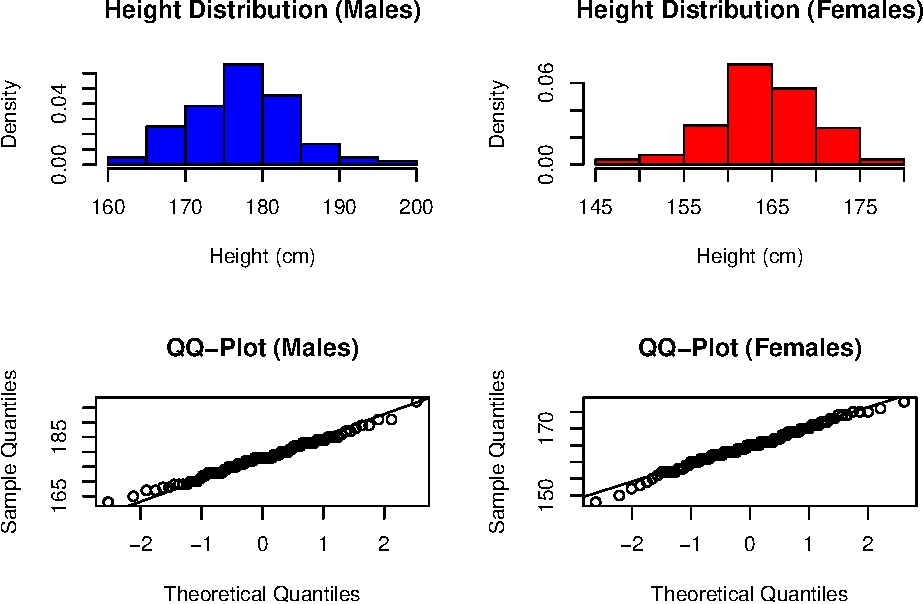
\includegraphics{SDA_submission_template_files/figure-latex/unnamed-chunk-2-1.pdf}

\begin{Shaded}
\begin{Highlighting}[]
\CommentTok{\# Normality test using Shapiro{-}Wilk}
\FunctionTok{shapiro.test}\NormalTok{(Davis\_M}\SpecialCharTok{$}\NormalTok{height)}
\end{Highlighting}
\end{Shaded}

\begin{verbatim}
## 
##  Shapiro-Wilk normality test
## 
## data:  Davis_M$height
## W = 0.99196, p-value = 0.872
\end{verbatim}

\begin{Shaded}
\begin{Highlighting}[]
\FunctionTok{shapiro.test}\NormalTok{(Davis\_F}\SpecialCharTok{$}\NormalTok{height)}
\end{Highlighting}
\end{Shaded}

\begin{verbatim}
## 
##  Shapiro-Wilk normality test
## 
## data:  Davis_F$height
## W = 0.98947, p-value = 0.5468
\end{verbatim}

from both the histograms and the qq-plots, we can see the distributions
of heights of both male and female are both close to normal
distribution. There are some wiggles observed in qq-plots, but they are
likely from rounding effect, not necessarily linked to unnormality. From
the histograms, we can observe a subtlety that heights of males have
more mass below the mean and vice versa for weights of females.

From Shapiro-Wilk test results, the null hypothesis is not rejected.

\subsection{b.}\label{b.}

\begin{Shaded}
\begin{Highlighting}[]
\CommentTok{\# Set seed for reproducibility}
\FunctionTok{set.seed}\NormalTok{(}\DecValTok{1234}\NormalTok{)}

\CommentTok{\# Function to compute the difference in means}
\NormalTok{mean\_diff }\OtherTok{\textless{}{-}} \ControlFlowTok{function}\NormalTok{(data) \{}
  \FunctionTok{mean}\NormalTok{(data}\SpecialCharTok{$}\NormalTok{height[data}\SpecialCharTok{$}\NormalTok{sex }\SpecialCharTok{==} \StringTok{"M"}\NormalTok{]) }\SpecialCharTok{{-}} \FunctionTok{mean}\NormalTok{(data}\SpecialCharTok{$}\NormalTok{height[data}\SpecialCharTok{$}\NormalTok{sex }\SpecialCharTok{==} \StringTok{"F"}\NormalTok{])}
\NormalTok{\}}

\CommentTok{\# **Empirical Bootstrap**}
\NormalTok{n\_bootstrap }\OtherTok{\textless{}{-}} \DecValTok{1000}  \CommentTok{\# Number of bootstrap samples}
\NormalTok{boot\_diffs\_empirical }\OtherTok{\textless{}{-}} \FunctionTok{replicate}\NormalTok{(n\_bootstrap, \{}
\NormalTok{  resample\_M }\OtherTok{\textless{}{-}} \FunctionTok{sample}\NormalTok{(Davis\_M}\SpecialCharTok{$}\NormalTok{height, }\AttributeTok{replace =} \ConstantTok{TRUE}\NormalTok{)}
\NormalTok{  resample\_F }\OtherTok{\textless{}{-}} \FunctionTok{sample}\NormalTok{(Davis\_F}\SpecialCharTok{$}\NormalTok{height, }\AttributeTok{replace =} \ConstantTok{TRUE}\NormalTok{)}
  \FunctionTok{mean}\NormalTok{(resample\_M) }\SpecialCharTok{{-}} \FunctionTok{mean}\NormalTok{(resample\_F)}
\NormalTok{\})}

\CommentTok{\# Standard deviation of bootstrap samples (empirical bootstrap)}
\NormalTok{sd\_empirical }\OtherTok{\textless{}{-}} \FunctionTok{sd}\NormalTok{(boot\_diffs\_empirical)}

\CommentTok{\# **Parametric Bootstrap (assuming normality)**}
\NormalTok{parametric\_boot\_diffs }\OtherTok{\textless{}{-}} \FunctionTok{replicate}\NormalTok{(n\_bootstrap, \{}
\NormalTok{  resample\_M }\OtherTok{\textless{}{-}} \FunctionTok{rnorm}\NormalTok{(}\FunctionTok{length}\NormalTok{(Davis\_M}\SpecialCharTok{$}\NormalTok{height), }\FunctionTok{mean}\NormalTok{(Davis\_M}\SpecialCharTok{$}\NormalTok{height), }\FunctionTok{sd}\NormalTok{(Davis\_M}\SpecialCharTok{$}\NormalTok{height))}
\NormalTok{  resample\_F }\OtherTok{\textless{}{-}} \FunctionTok{rnorm}\NormalTok{(}\FunctionTok{length}\NormalTok{(Davis\_F}\SpecialCharTok{$}\NormalTok{height), }\FunctionTok{mean}\NormalTok{(Davis\_F}\SpecialCharTok{$}\NormalTok{height), }\FunctionTok{sd}\NormalTok{(Davis\_F}\SpecialCharTok{$}\NormalTok{height))}
  \FunctionTok{mean}\NormalTok{(resample\_M) }\SpecialCharTok{{-}} \FunctionTok{mean}\NormalTok{(resample\_F)}
\NormalTok{\})}

\CommentTok{\# Standard deviation of bootstrap samples (parametric bootstrap)}
\NormalTok{sd\_parametric }\OtherTok{\textless{}{-}} \FunctionTok{sd}\NormalTok{(parametric\_boot\_diffs)}

\CommentTok{\# Print results}
\FunctionTok{cat}\NormalTok{(}\StringTok{"Empirical Bootstrap SD:"}\NormalTok{, sd\_empirical, }\StringTok{"}\SpecialCharTok{\textbackslash{}n}\StringTok{"}\NormalTok{)}
\end{Highlighting}
\end{Shaded}

\begin{verbatim}
## Empirical Bootstrap SD: 0.8418963
\end{verbatim}

\begin{Shaded}
\begin{Highlighting}[]
\FunctionTok{cat}\NormalTok{(}\StringTok{"Parametric Bootstrap SD:"}\NormalTok{, sd\_parametric, }\StringTok{"}\SpecialCharTok{\textbackslash{}n}\StringTok{"}\NormalTok{)}
\end{Highlighting}
\end{Shaded}

\begin{verbatim}
## Parametric Bootstrap SD: 0.8904208
\end{verbatim}

\subsection{c.}\label{c.}

\begin{Shaded}
\begin{Highlighting}[]
\CommentTok{\# Given values}
\NormalTok{mu\_M }\OtherTok{\textless{}{-}} \FloatTok{177.8}
\NormalTok{mu\_F }\OtherTok{\textless{}{-}} \FloatTok{164.6}
\NormalTok{sigma\_M }\OtherTok{\textless{}{-}} \FloatTok{6.5}
\NormalTok{sigma\_F }\OtherTok{\textless{}{-}} \FloatTok{5.5}
\NormalTok{n\_M }\OtherTok{\textless{}{-}} \FunctionTok{length}\NormalTok{(Davis\_M}\SpecialCharTok{$}\NormalTok{height)}
\NormalTok{n\_F }\OtherTok{\textless{}{-}} \FunctionTok{length}\NormalTok{(Davis\_F}\SpecialCharTok{$}\NormalTok{height)}

\CommentTok{\# Compute theoretical standard deviation}
\NormalTok{theoretical\_sd }\OtherTok{\textless{}{-}} \FunctionTok{sqrt}\NormalTok{((sigma\_M}\SpecialCharTok{\^{}}\DecValTok{2} \SpecialCharTok{/}\NormalTok{ n\_M) }\SpecialCharTok{+}\NormalTok{ (sigma\_F}\SpecialCharTok{\^{}}\DecValTok{2} \SpecialCharTok{/}\NormalTok{ n\_F))}
\FunctionTok{cat}\NormalTok{(}\StringTok{"Theoretical SD:"}\NormalTok{, theoretical\_sd, }\StringTok{"}\SpecialCharTok{\textbackslash{}n}\StringTok{"}\NormalTok{)}
\end{Highlighting}
\end{Shaded}

\begin{verbatim}
## Theoretical SD: 0.8675461
\end{verbatim}

\begin{Shaded}
\begin{Highlighting}[]
\CommentTok{\# Compare theoretical vs. bootstrap estimates}
\NormalTok{comparison }\OtherTok{\textless{}{-}} \FunctionTok{data.frame}\NormalTok{(}
  \AttributeTok{Method =} \FunctionTok{c}\NormalTok{(}\StringTok{"Empirical Bootstrap"}\NormalTok{, }\StringTok{"Parametric Bootstrap"}\NormalTok{, }\StringTok{"Theoretical"}\NormalTok{),}
  \AttributeTok{SD =} \FunctionTok{c}\NormalTok{(sd\_empirical, sd\_parametric, theoretical\_sd)}
\NormalTok{)}

\FunctionTok{print}\NormalTok{(comparison)}
\end{Highlighting}
\end{Shaded}

\begin{verbatim}
##                 Method        SD
## 1  Empirical Bootstrap 0.8418963
## 2 Parametric Bootstrap 0.8904208
## 3          Theoretical 0.8675461
\end{verbatim}

the parametric boostrap estimation of the sd of the mean difference is
closer to the theoretical value

\subsection{d.}\label{d.}

\begin{Shaded}
\begin{Highlighting}[]
\CommentTok{\# Set boundaries for uniform distribution}
\NormalTok{min\_M }\OtherTok{\textless{}{-}} \FunctionTok{min}\NormalTok{(Davis\_M}\SpecialCharTok{$}\NormalTok{height)}
\NormalTok{max\_M }\OtherTok{\textless{}{-}} \FunctionTok{max}\NormalTok{(Davis\_M}\SpecialCharTok{$}\NormalTok{height)}
\NormalTok{min\_F }\OtherTok{\textless{}{-}} \FunctionTok{min}\NormalTok{(Davis\_F}\SpecialCharTok{$}\NormalTok{height)}
\NormalTok{max\_F }\OtherTok{\textless{}{-}} \FunctionTok{max}\NormalTok{(Davis\_F}\SpecialCharTok{$}\NormalTok{height)}

\CommentTok{\# Perform parametric bootstrap with uniform distribution}
\NormalTok{uniform\_boot\_diffs }\OtherTok{\textless{}{-}} \FunctionTok{replicate}\NormalTok{(n\_bootstrap, \{}
\NormalTok{  resample\_M }\OtherTok{\textless{}{-}} \FunctionTok{runif}\NormalTok{(n\_M, min\_M, max\_M)}
\NormalTok{  resample\_F }\OtherTok{\textless{}{-}} \FunctionTok{runif}\NormalTok{(n\_F, min\_F, max\_F)}
  \FunctionTok{mean}\NormalTok{(resample\_M) }\SpecialCharTok{{-}} \FunctionTok{mean}\NormalTok{(resample\_F)}
\NormalTok{\})}

\CommentTok{\# Standard deviation of bootstrap samples (uniform distribution)}
\NormalTok{sd\_uniform }\OtherTok{\textless{}{-}} \FunctionTok{sd}\NormalTok{(uniform\_boot\_diffs)}

\FunctionTok{cat}\NormalTok{(}\StringTok{"Uniform Bootstrap SD:"}\NormalTok{, sd\_uniform, }\StringTok{"}\SpecialCharTok{\textbackslash{}n}\StringTok{"}\NormalTok{)}
\end{Highlighting}
\end{Shaded}

\begin{verbatim}
## Uniform Bootstrap SD: 1.313566
\end{verbatim}

\begin{Shaded}
\begin{Highlighting}[]
\CommentTok{\# Compare with theoretical standard deviation}
\NormalTok{comparison }\OtherTok{\textless{}{-}} \FunctionTok{rbind}\NormalTok{(comparison, }\FunctionTok{c}\NormalTok{(}\StringTok{"Uniform Bootstrap"}\NormalTok{, sd\_uniform))}
\FunctionTok{print}\NormalTok{(comparison)}
\end{Highlighting}
\end{Shaded}

\begin{verbatim}
##                 Method                SD
## 1  Empirical Bootstrap 0.841896285568105
## 2 Parametric Bootstrap 0.890420792940573
## 3          Theoretical 0.867546055772349
## 4    Uniform Bootstrap  1.31356582282602
\end{verbatim}

\section{Exercise 2}\label{exercise-2}

\subsection{a.}\label{a.-1}

It is given that
\[\tilde{D_n}=max_i max\left(\left| \frac{i-1}{n} - \Phi\left( \frac{X_{(i)}-\bar{X}}{S} \right)\right|, \left| \frac{i}{n} - \Phi\left(\frac{X_{(i)}-\bar{X}}{S}\right) \right|\right)\]

This depends on \(F\) by using \(\frac{X_{(i)}-\bar{X}}{S}\) and the
null hypothesis states that \(X_{(i)}\sim N(\bar{X},S)\). Thus
\(X_{(i)}-\bar{X}\sim N(0,S)\) and finally we define
\(Z_{(i)}=\frac{X_{(i)}-\bar{X}}{S}\sim N(0,1)\). Substituting this in
our original equation we get:
\[\tilde{D_n}=max_i max\left(\left| \frac{i-1}{n} - \Phi\left(Z_{(i)} \right)\right|, \left| \frac{i}{n} - \Phi\left(Z_{(i)}\right) \right|\right)\]
Which shows that under the null, \(\tilde{D}_n\) is independent of the
location and scale parameters since \(Z_{(i)}\) is independent of them.

\subsection{b.}\label{b.-1}

\begin{Shaded}
\begin{Highlighting}[]
\CommentTok{\# Load the data}
\FunctionTok{data}\NormalTok{(morley)}
\FunctionTok{head}\NormalTok{(morley)}
\end{Highlighting}
\end{Shaded}

\begin{verbatim}
##     Expt Run Speed
## 001    1   1   850
## 002    1   2   740
## 003    1   3   900
## 004    1   4  1070
## 005    1   5   930
## 006    1   6   850
\end{verbatim}

\begin{Shaded}
\begin{Highlighting}[]
\NormalTok{l\_speed }\OtherTok{\textless{}{-}}\NormalTok{ morley}\SpecialCharTok{$}\NormalTok{Speed}

\CommentTok{\# Calculate the mean and standard dev}
\NormalTok{m\_speed }\OtherTok{\textless{}{-}} \FunctionTok{mean}\NormalTok{(l\_speed)}
\NormalTok{sd\_speed }\OtherTok{\textless{}{-}} \FunctionTok{sd}\NormalTok{(l\_speed)}

\CommentTok{\# run ks.test}
\NormalTok{ks\_result }\OtherTok{\textless{}{-}} \FunctionTok{ks.test}\NormalTok{(l\_speed, }\StringTok{"pnorm"}\NormalTok{, }\AttributeTok{mean =}\NormalTok{ m\_speed, }\AttributeTok{sd =}\NormalTok{ sd\_speed)}
\end{Highlighting}
\end{Shaded}

\begin{verbatim}
## Warning in ks.test.default(l_speed, "pnorm", mean = m_speed, sd = sd_speed):
## ties should not be present for the one-sample Kolmogorov-Smirnov test
\end{verbatim}

\begin{Shaded}
\begin{Highlighting}[]
\CommentTok{\# Extract D\_n and the p{-}value}
\NormalTok{D\_n }\OtherTok{\textless{}{-}}\NormalTok{ ks\_result}\SpecialCharTok{$}\NormalTok{statistic}
\NormalTok{p\_value }\OtherTok{\textless{}{-}}\NormalTok{ ks\_result}\SpecialCharTok{$}\NormalTok{p.value}
\FunctionTok{print}\NormalTok{(D\_n)}
\end{Highlighting}
\end{Shaded}

\begin{verbatim}
##          D 
## 0.08342437
\end{verbatim}

\begin{Shaded}
\begin{Highlighting}[]
\FunctionTok{print}\NormalTok{(p\_value)}
\end{Highlighting}
\end{Shaded}

\begin{verbatim}
## [1] 0.4895616
\end{verbatim}

The p-value (0.4895616) is more than the significance level of 0.05 and
thus we don't reject the null hypothesis that the data follows a normal
distribution. The p-value isn't reliable since the Kolmogorov-Smirnov
assumes that we now the parameters of the distribution, but we had to
estimate them using the sample mean and standard deviation. (R also
gives the warning ``Warning: ties should not be present for the
one-sample Kolmogorov-Smirnov test'' which means that some values in the
data repeat which and that shouldn't happen since the test is made for a
continuous distribution.)

\subsection{c.}\label{c.-1}

\begin{Shaded}
\begin{Highlighting}[]
\FunctionTok{set.seed}\NormalTok{(}\DecValTok{1234}\NormalTok{)}

\NormalTok{n }\OtherTok{\textless{}{-}} \FunctionTok{length}\NormalTok{(l\_speed)}
\NormalTok{B }\OtherTok{\textless{}{-}} \DecValTok{1000}
\NormalTok{Dn\_star }\OtherTok{\textless{}{-}} \FunctionTok{numeric}\NormalTok{(B)}

\ControlFlowTok{for}\NormalTok{ (i }\ControlFlowTok{in} \DecValTok{1}\SpecialCharTok{:}\NormalTok{B) \{}
  \CommentTok{\# Generate bootstrap sample from N(m\_speed, sd\_speed\^{}2)}
\NormalTok{  bootstrap\_sample }\OtherTok{\textless{}{-}} \FunctionTok{rnorm}\NormalTok{(n, }\AttributeTok{mean =}\NormalTok{ m\_speed, }\AttributeTok{sd =}\NormalTok{ sd\_speed)}

  \CommentTok{\# Calculate the mean and standard dev}
\NormalTok{  m\_star }\OtherTok{\textless{}{-}} \FunctionTok{mean}\NormalTok{(bootstrap\_sample)}
\NormalTok{  sd\_star }\OtherTok{\textless{}{-}} \FunctionTok{sd}\NormalTok{(bootstrap\_sample)}
  
  \CommentTok{\# run ks.test}
\NormalTok{  ks\_star }\OtherTok{\textless{}{-}} \FunctionTok{ks.test}\NormalTok{(bootstrap\_sample, }\StringTok{"pnorm"}\NormalTok{, }\AttributeTok{mean =}\NormalTok{ m\_star, }\AttributeTok{sd =}\NormalTok{ sd\_star)}
\NormalTok{  Dn\_star[i] }\OtherTok{\textless{}{-}}\NormalTok{ ks\_star}\SpecialCharTok{$}\NormalTok{statistic}
\NormalTok{\}}

\CommentTok{\# compute p{-}value using the bootstrap distribution}
\NormalTok{p\_value\_bootstrap }\OtherTok{\textless{}{-}} \FunctionTok{mean}\NormalTok{(Dn\_star }\SpecialCharTok{\textgreater{}=}\NormalTok{ D\_n)}

\FunctionTok{print}\NormalTok{(p\_value\_bootstrap)}
\end{Highlighting}
\end{Shaded}

\begin{verbatim}
## [1] 0.078
\end{verbatim}

\subsection{d.}\label{d.-1}

There is a big difference between the p-values in b and c.~b results in
a p-value of 0.4895616 and the bootstrap method in c results in a
p-value of 0.078. This difference of 0.411 is very big, but still not
large enough to result in different test decisions as the result from c
is still above the significance level of 0.05. The final conclusion is
that both tests result in not rejecting the null hypothesis and thus not
having enough evidence that the data doesn't follow a normal
distribution.

\end{document}
